\paragraph{CPSs (1)}

The graph below is a constraint graph for a CSP that has only binary constraints. Initially, no variables have been assigned.
\\\\
For each of the following scenarios, mark all variables for which the specified filtering might result in their domain being changed. 

\begin{center}
    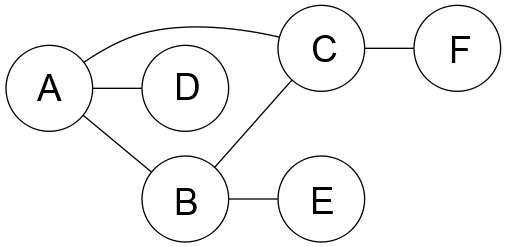
\includegraphics[scale=.43]{figures/domainFiltering.png}
\end{center}



\begin{enumerate}

\item A value is assigned to A. Which domains might be changed as a result of running forward checking for A? (\textbf{10 points})

{\color{red} B\&C\&D. Forward checking for A only considers arcs where A is the head. This includes $B\rightarrow A$, $C\rightarrow A$, $D\rightarrow A$. Enforcing these arcs can change the domains of the tails.
}

\item A value is assigned to A, and then forward checking is run for A. Then a value is assigned to B. Which domains might be changed as a result of running forward checking for B? (\textbf{10 points})

{\color{red} C\&E. Similar to the previous part, forward checking for $B$ enforces the arcs $A\rightarrow B$, $C\rightarrow B$, and $E\rightarrow B$. However, because $A$ has been assigned, and a value is assigned to $B$, which is consistent with $A$ or else no value would have been assigned, the domain of $A$ will not change.}

\item A value is assigned to A. Which domains might be changed as a result of enforcing arc consistency after this assignment? (\textbf{10 points})

{\color{red} B\&C\&D\&E\&F. Enforcing arc consistency can affect any unassigned variable in the graph that has a path to the assigned variable. This is because a change to the domain of $X$ results in enforcing all arcs where $X$ is the head, so changes propagate through the graph. Note that the only time in which the domain for $A$ changes is if any domain becomes empty, in which case the arc consistency algorithm usually returns immediately and backtracking is required, so it does not really make sense to consider new domains in this case.}


\item A value is assigned to A, and then arc consistency is enforced. Then a value is assigned to B. Which domains might be changed as a result of enforcing arc consistency after the assignment to B? (\textbf{10 points})

{\color{red} C\&E\&F. After assigning a value to $A$, and enforcing arc consistency, future assignments and enforcing arc consistency will not result in a change to $A$s domain. This means that $D$s domain won't change because the only arc that might cause a change, $D\rightarrow A$ will never be enforced.}

\end{enumerate}

\newpage

\paragraph{CPSs (2)}

After years of struggling through mazes, Pacman has finally made peace with the ghosts, Blinky, Pinky, Inky, and Clyde, and invited them to live with him and Ms. Pacman. The move has forced Pacman to change the rooming assignments in his house, which has 6 rooms. He has decided to figure out the new assignments with a CSP in which the variables are Pacman \textbf{(P)}, Ms. Pacman \textbf{(M)}, Blinky \textbf{(B)}, Pinky \textbf{(K)}, Inky \textbf{(I)}, and Clyde \textbf{(C)}, the values are which room they will stay in, from 1-6, and the constraints are:\\
\begin{table}[h]
\centering
\caption{Constraints}
\begin{tabular}{ll}
i) No two agents can stay in the same room&\\
ii) \textbf{P} $>$ 3 &
vi) \textbf{B} is even\\
iii) \textbf{K} is less than \textbf{P}&
vii) \textbf{I} is not 1 or 6\\
iv) \textbf{M} is either 5 or 6&
viii) $\vert$\textbf{I}-\textbf{C}$\vert$ = 1\\
v) \textbf{P} $>$ \textbf{M}&
ix) $\vert$\textbf{P}-\textbf{B}$\vert$ = 2
\end{tabular}
\end{table}


\begin{enumerate}
  \item {\bf Unary constraints} On the grid below cross out the values from each domain that are eliminated by enforcing unary constraints. (\textbf{10 points})

  \begin{table}[h]
\centering
\caption{}
\begin{tabular}{ccccccc}
P & {\color{red}\sout{1}} & {\color{red}\sout{2} }& {\color{red}\sout{3}} & 4 & 5 & 6\\
B & {\color{red}\sout{1} }& 2 & {\color{red}\sout{3}} & 4 & {\color{red}\sout{5}} & 6\\
C & 1 & 2 & 3 & 4 & 5 & 6\\
K & 1 & 2 & 3 & 4 & 5 & 6\\
I & {\color{red}\sout{1}} & 2 & 3 & 4 & 5 & {\color{red}\sout{6}}\\
M & {\color{red}\sout{1}} & {\color{red}\sout{2}} & {\color{red}\sout{3}} & {\color{red}\sout{4}} & 5 & 6\\
\end{tabular}
\end{table}

{\color{red} The unary constraints are ii, iv, vi, and vii. ii crosses out 1,2, and 3 for P. iv crosses out 1,2,3,4 for M. vi crosses out 1,3, and 5 for B. vii crosses out 1 and 6 for I. K and C have no unary constraints, so their domains remain the same.}


\item {\bf MRV}
According to the Minimum Remaining Value (MRV) heuristic, which variable should be assigned to first? (\textbf{10 points})

{\color{red} M has the fewest value remaining in its domain (2), so it should be selected first for assignment.
}
\newpage

\item {\bf Forward Checking}
For the purposes of decoupling this problem from your solution to the
previous problem, assume we choose to assign P first, and assign it the value 6. What are the resulting domains after enforcing unary constraints (from part i) and running forward checking for this assignment? (\textbf{15 points})

\begin{table}[h]
\centering
\caption{}
\begin{tabular}{ccccccc}
P &   &   &   &  &   &  6\\
B & {\color{red}\sout{1}} & {\color{red}\sout{2}} & {\color{red}\sout{3}} & 4 & {\color{red}\sout{5}} & {\color{red}\sout{6}}\\
C & 1 & 2 & 3 & 4 & 5 & {\color{red}\sout{6}}\\
K & 1 & 2 & 3 & 4 & 5 & {\color{red}\sout{6}}\\
I & {\color{red}\sout{1}} & 2 & 3 & 4 & 5 & {\color{red}\sout{6}}\\
M & {\color{red}\sout{1}} &{\color{red} \sout{2}} & {\color{red}\sout{3}} & {\color{red}\sout{4}} & 5 & {\color{red}\sout{6}}\\
\end{tabular}
\end{table}

{\color{red} In addition to enforcing the unary constraints from part i, the domains are further constrained by all constraints involving P. This includes constraints i, iii, v, and ix. i removes 6 from the domains of all variables. iii removes 6 from the domain of K (already removed by constraint i). v removes 6 from the domain of M (also already removed by i). ix removes 2 and 6 from the domain of B. 
}

\item {\bf Iterative Improvement}
Instead of running backtracking search, you decide to start over and run
iterative improvement with the min-conflicts heuristic for value selection. Starting with the following assignment:\\\\
P:6, B:4, C:3, K:2, I:1, M:5\\\\
First, for each variable write down how many constraints it violates in the table below.\\
Then, in the table on the right, for all variables that could be selected for assignment, put an x in any box that corresponds to a possible value that could be assigned to that variable according to min-conflicts. When marking next values a variable could take on, only mark values different from the current one. (\textbf{25 points})

\begin{center}
\begin{tabular}{cc}
\begin{tabular}{|c|c|}
\hline
Variable & \# violated\\
\hline
P& {\color{red}0}\\
\hline
B& {\color{red}0}\\
\hline
C& {\color{red}1}\\
\hline
K& {\color{red}0}\\
\hline
I& {\color{red}2}\\
\hline
M& {\color{red}0}\\
\hline
\end{tabular} \hspace{2cm}&
\begin{tabular}{|c|c|c|c|c|c|c|}
\hline
&1&2&3&4&5&6\\
\hline
P& & & & & &\\
\hline
B& & & & & &\\
\hline
C& & {\color{red}x}& & & &\\
\hline
K& & & & & &\\
\hline
I& &  {\color{red}x}& & {\color{red}x} & &\\
\hline
M& & & & & &\\
\hline
\end{tabular}
\end{tabular}
\end{center}

{\color{red} Both I and C violate constraint viii, because $\vert$I-C$\vert$=2. I also violates constraint vii. No other variables violate any constraints. According to iterative improvement, any conflicted variable could be selected for assignment, in this case I and C. According to min-conflicts, the values that those variables can take on are the values that minimize the number of constraints violated by the variable. Assigning 2 or 4 to I causes it to violate constraint i, because other variables already have the values 2 and 4. Assigning 2 to C also only causes C to violate 1 constraint.
}

\end{enumerate}